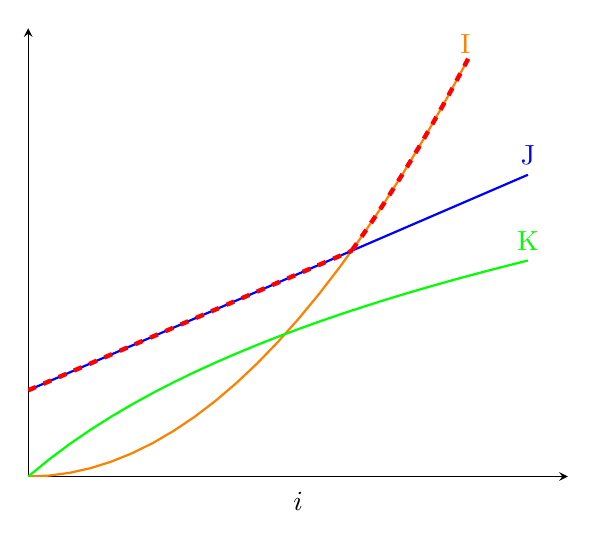
\begin{tikzpicture}
\begin{axis}[
    axis lines = left,
    xlabel = \(i\),
    ylabel = {},
    domain = 0:2.5,
    xtick={\empty},ytick={\empty},
    ymin=0,
    ymax=5.2,
    xmax=2.7,
    restrict y to domain=0:5,
]
    \addplot[thick, color=orange]{x^2} node[above,pos=1] {I};
    \addplot[thick, color=blue]{x+1} node[above,pos=1] {J};
    \addplot[thick, color=green]{ln(x+1)*2} node[above,pos=1] {K};
    \draw [ultra thick, dashed, draw=red] (axis cs:0,1) -- (axis cs:1.62,2.62);
    \addplot[ultra thick, color=green, dashed, color=red, domain=1.62:2.5]{x^2};
\end{axis}
\end{tikzpicture}